\chapter{Initial Knowledge和Axiom}
Initial Knowledge和Axiom用于维护协议中的一些先验知识,其中Initial Knowledge指示进程模板中的哪些Attribute是对外公开可用的,而Axiom用于书写公理公式。

\section{Initial Knowledge}
在[协议>概览]下,点击小工具栏上的[创建InitialKnowledge]按钮,即可创建新的InitialKnowledge的类图,如图\ref{create_ik}所示。
\begin{figure}[h]
	\centering
	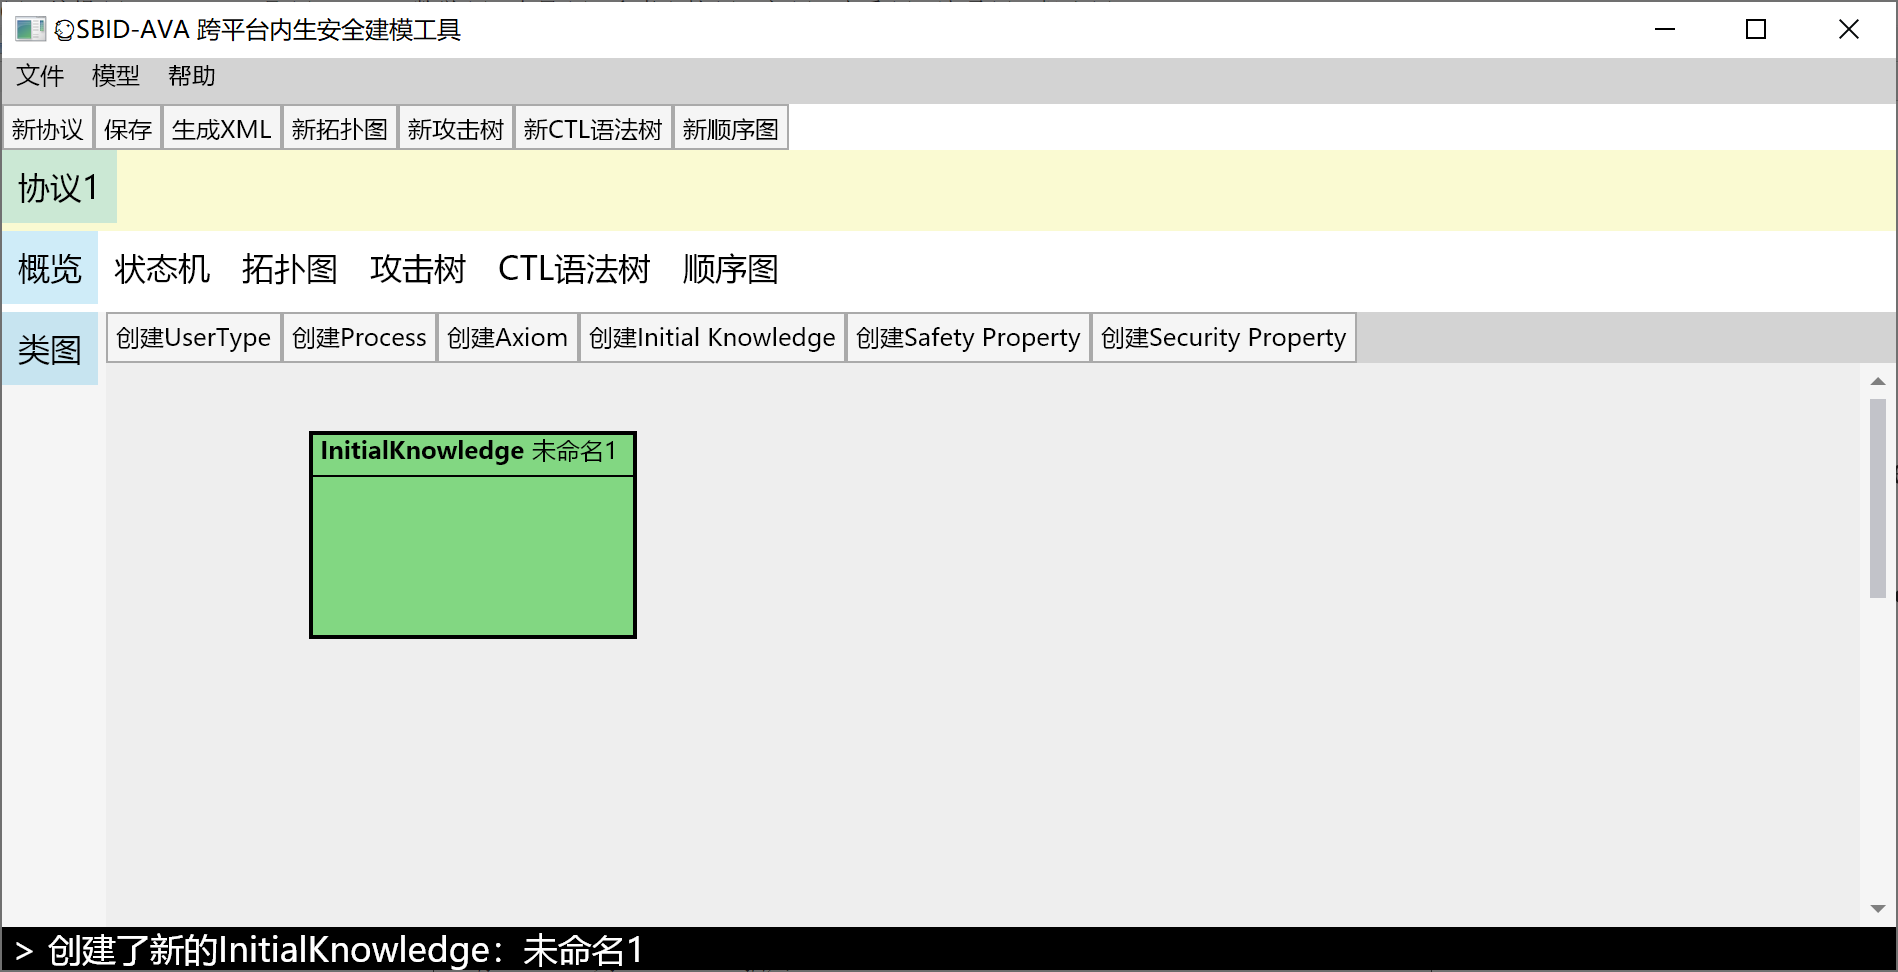
\includegraphics[width=12cm,height=6.75cm]{imgs/create_ik.png}
	\caption{新创建的InitialKnowledge}
	\label{create_ik}
\end{figure}
\par
在类图上右键,选择[编辑],即可打开InitialKnowledge的编辑对话框。调整到[KnowledgePair]选项卡中,可以操作协议中已添加的进程模板以及该进程模板下的Attribute,以作为该进程模板的InitialKnowledge之一,如图\ref{edit_ik}所示。
\begin{figure}[h]
	\centering
	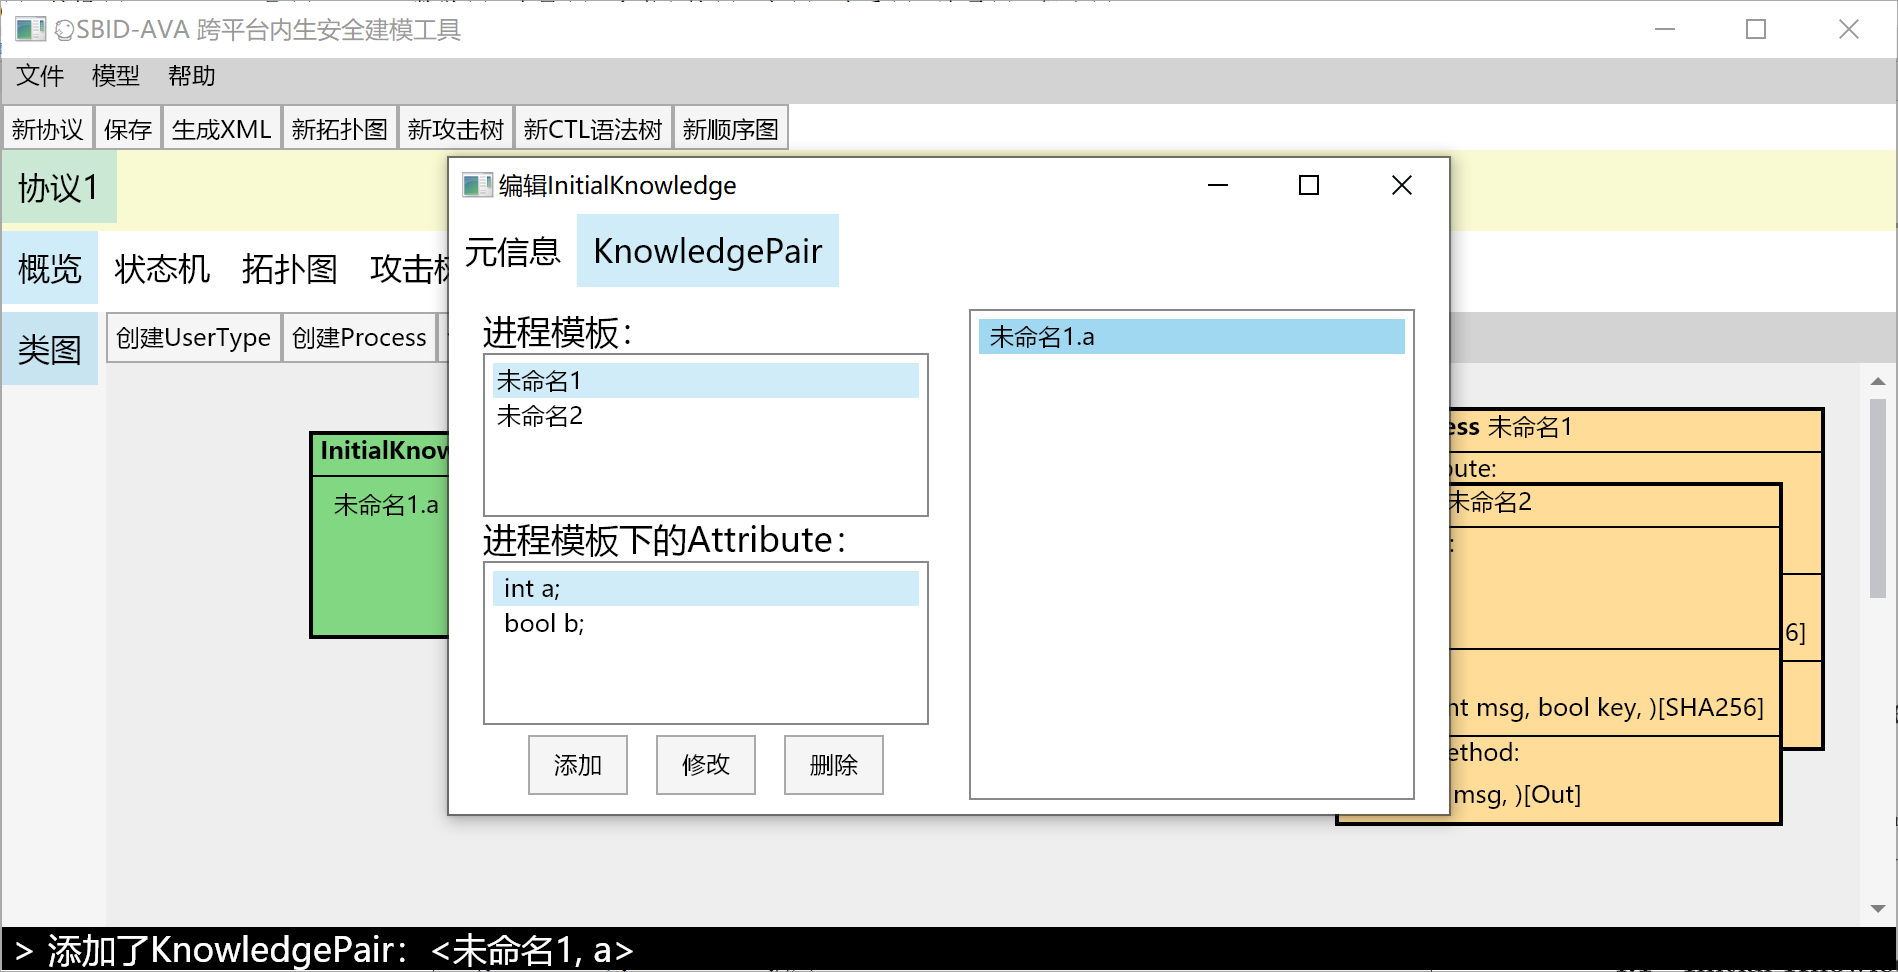
\includegraphics[width=12cm,height=6.75cm]{imgs/edit_ik.png}
	\caption{编辑InitialKnowledge}
	\label{edit_ik}
\end{figure}
\par
所以,为协议添加进程模板及其Attribute是添加InitialKnowledge的前提。

\section{Axiom}
在[协议>概览]下,点击小工具栏上的[创建Axiom]按钮,即可创建新的Axiom的类图,如图\ref{create_axiom}所示。
\begin{figure}[h]
	\centering
	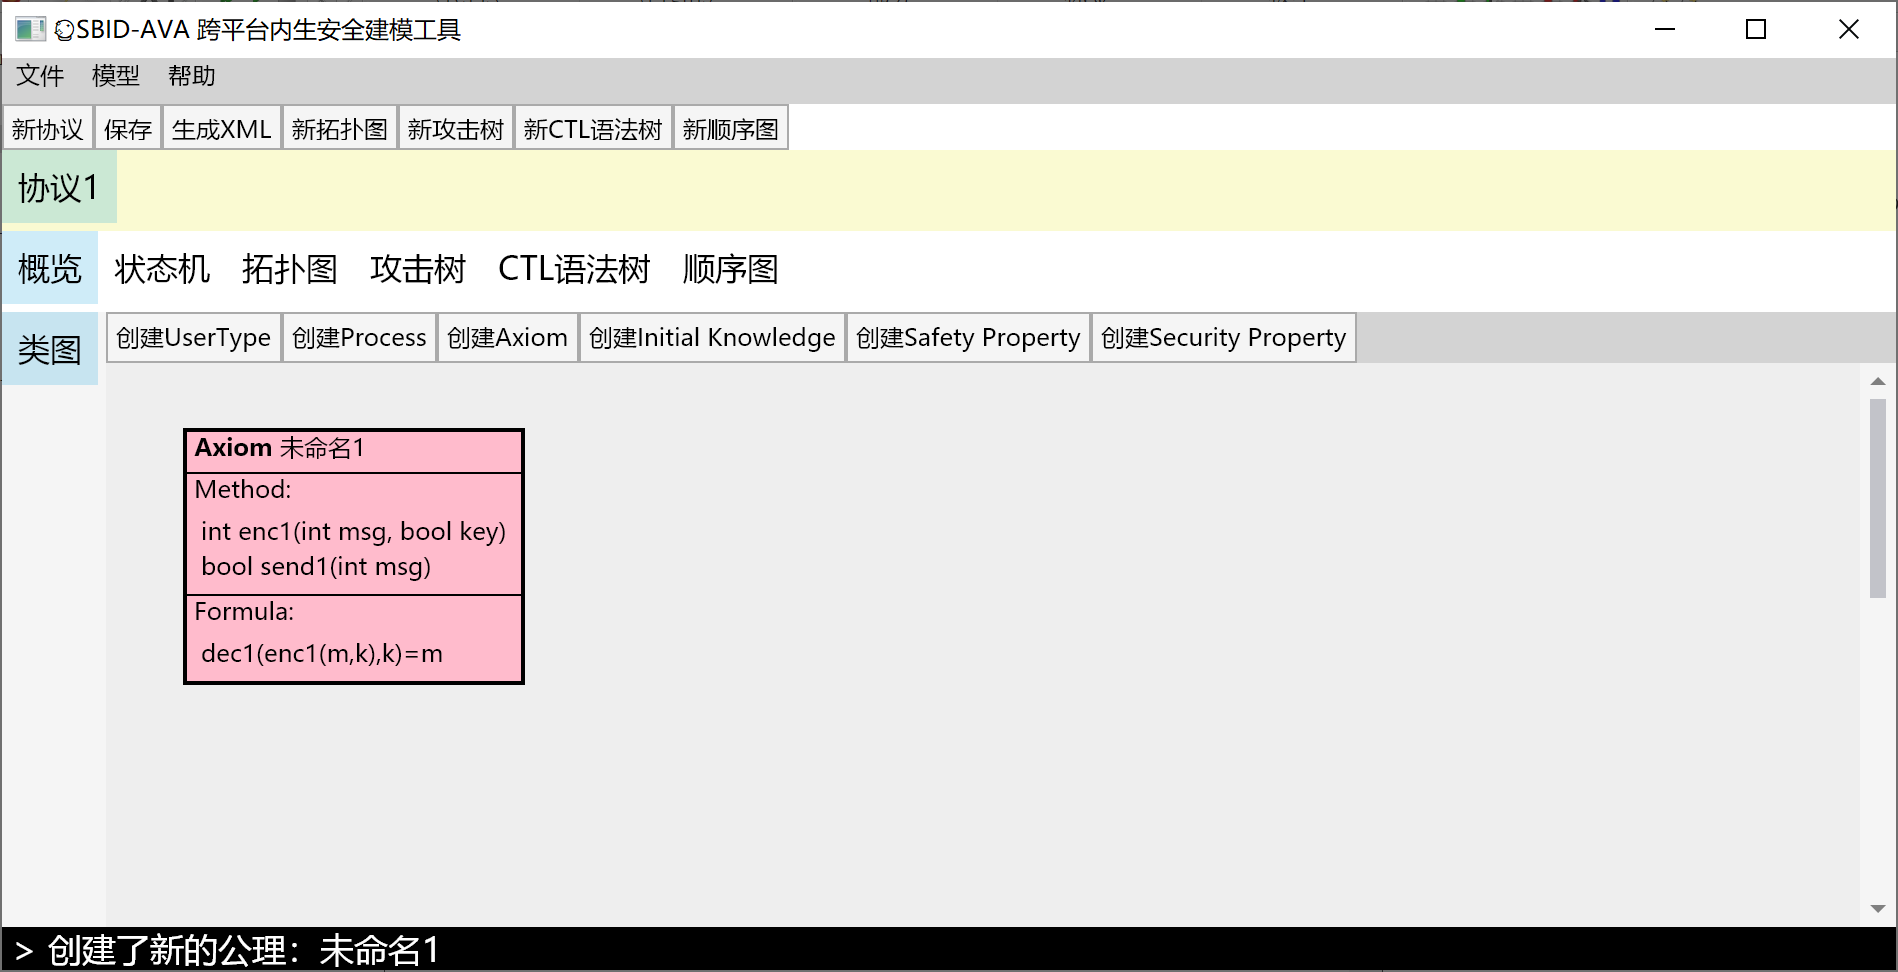
\includegraphics[width=12cm,height=6.75cm]{imgs/create_axiom.png}
	\caption{新创建的Axiom}
	\label{create_axiom}
\end{figure}
\par
在类图上右键,选择[编辑],即可打开Axiom的编辑对话框。调整到[Method]选项卡中,可以操作公理中的成员方法,如图\ref{edit_axiom_method}所示。
\begin{figure}[h]
	\centering
	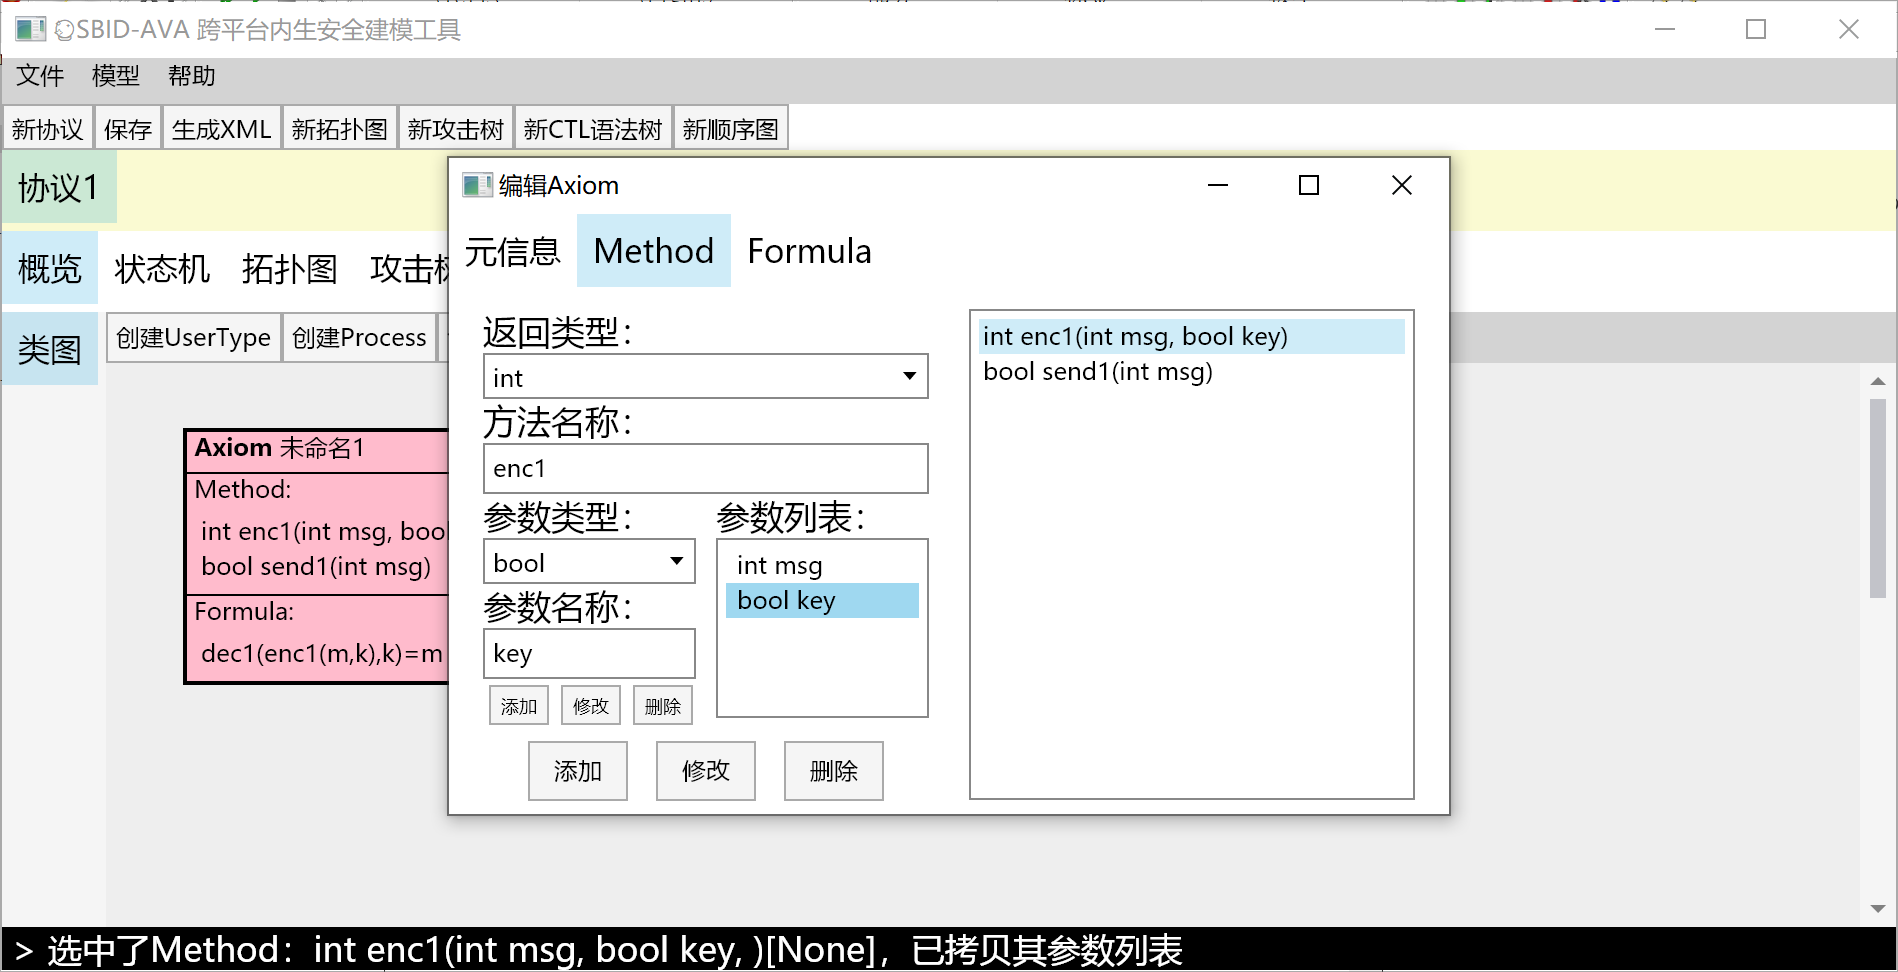
\includegraphics[width=12cm,height=6.75cm]{imgs/edit_axiom_method.png}
	\caption{编辑Axiom的Method}
	\label{edit_axiom_method}
\end{figure}
\par
调整到[Formula]选项卡中,可以操作公理公式,如图\ref{edit_axiom_formula}所示,表示公理中的两成员Method为一对加解密方法。
\begin{figure}[h]
	\centering
	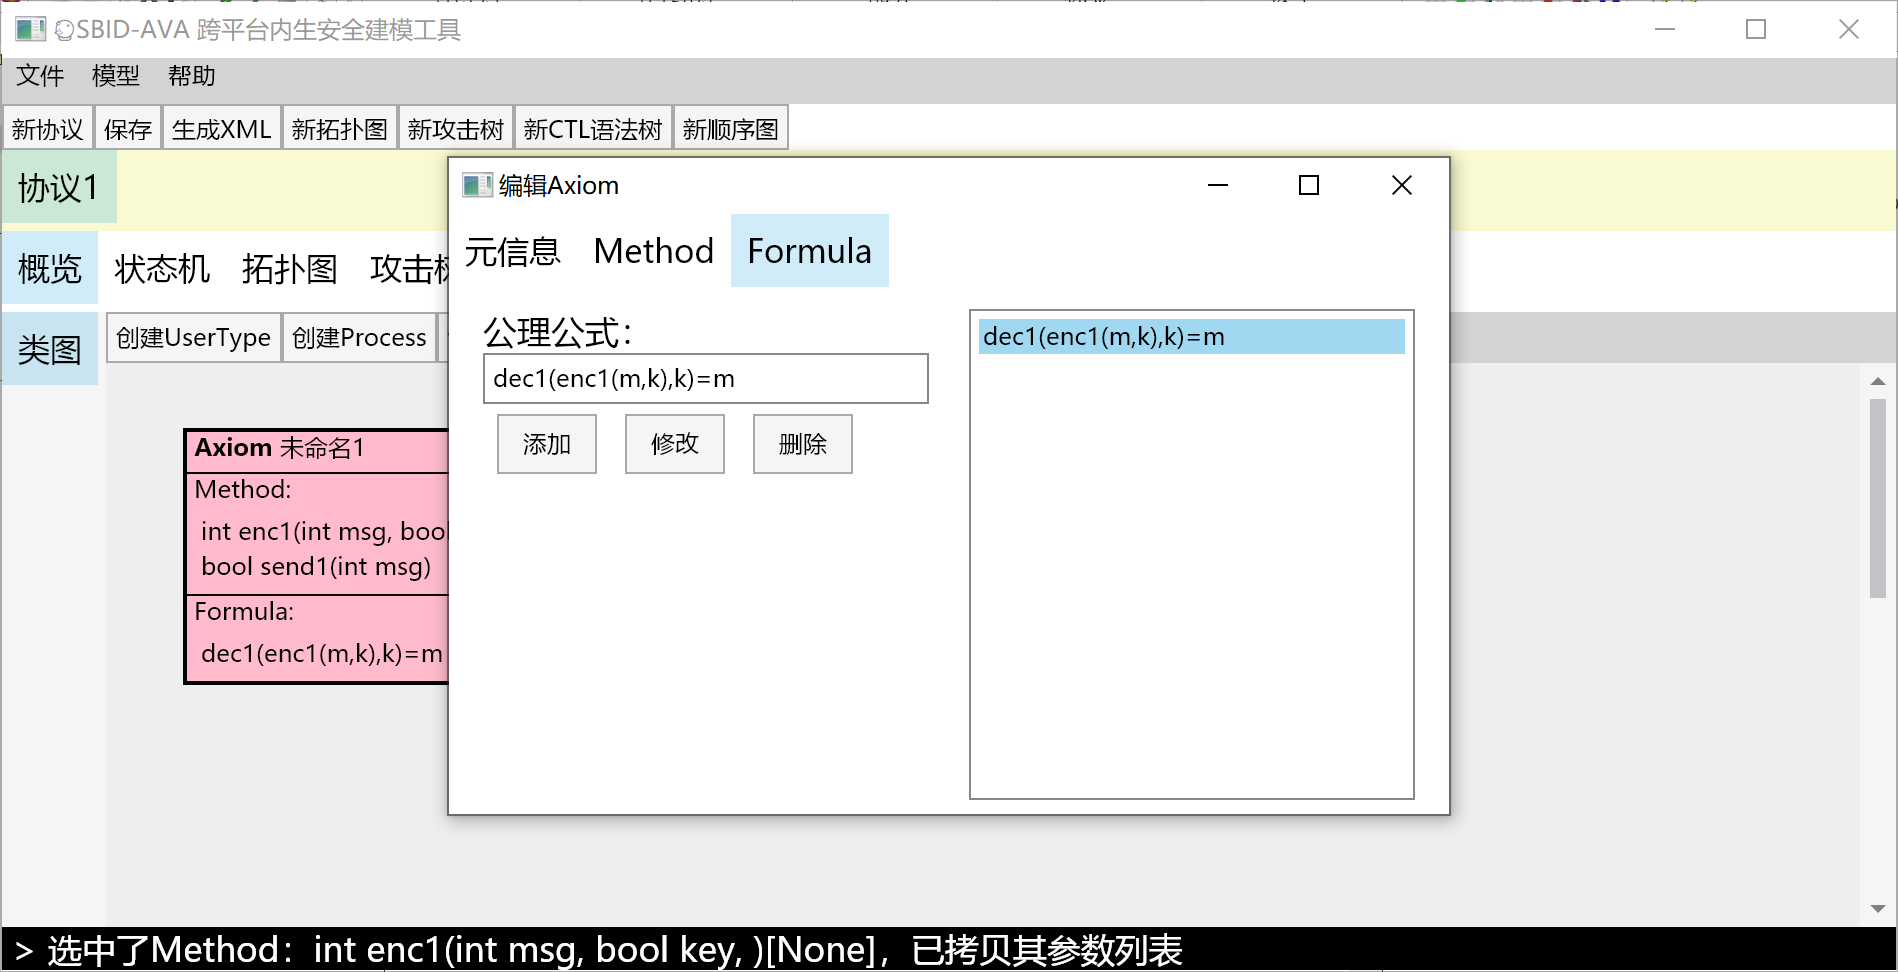
\includegraphics[width=12cm,height=6.75cm]{imgs/edit_axiom_formula.png}
	\caption{编辑Axiom的Formula}
	\label{edit_axiom_formula}
\end{figure}
